%%%%%%%%%%%%%%%%%%%%%%%%%%%%%%%%%%%%%%%%%%%%%%%%%%%
%% P3: Phenomenology of Particle Physics                         
%%
%% Author:  André Rubbia                   		 
%%
%% Figure 6.1 Illustration of the transformation of a vector field under  a rotation.
%%
%% This work is licensed under the Creative Commons Attribution 4.0 International License. 
%% To view a copy of this license, visit http://creativecommons.org/licenses/by/4.0/ or 
%% send a letter to Creative Commons, PO Box 1866, Mountain View, CA 94042, USA.
%%
%%%%%%%%%%%%%%%%%%%%%%%%%%%%%%%%%%%%%%%%%%%%%%%%%%%

\documentclass[a4paper,10pt]{article}

\usepackage[T1]{fontenc}
\usepackage[utf8]{inputenc}
\usepackage{lmodern}
\usepackage[labelfont=bf]{caption}
\usepackage{upgreek}

\usepackage{tikz}
\usepackage{pgfplots}
\pgfplotsset{compat=1.17}
\usepgfplotslibrary{ternary}
\usepgfplotslibrary{fillbetween}
\usepgfplotslibrary{external}

\def\d{\mathrm{d}}

\begin{document}

%%%%%%%%%%%%%%%   FIGURE  %%%%%%%%%%%%%%%%%%%%%%%%%%%%%%
\begin{figure}[htb]
    \centering
    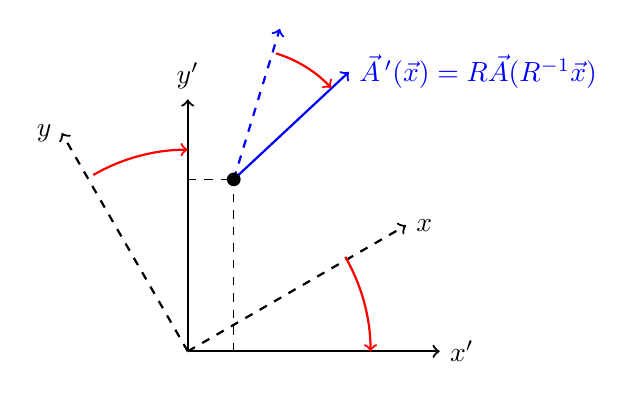
\begin{tikzpicture}[scale=0.8]
        \draw[thick,->] (6,0) -- (10,0) node[right] {$x'$};
        \draw[thick,->] (6,0) -- (6,4) node[above] {$y'$};
        \draw[dashed,thick,->] (6,0) -- +(120:4) node[left] {$y$};
        \draw[dashed,thick,->] (6,0) -- +(30:4) node[right] {$x$};
        \draw[dashed] (6,2.73) -- (6.73,2.73);
        \draw[dashed] (6.73,0) -- (6.73,2.73);
        \draw[blue,thick,->]  (6.73,2.73) -- +(43:2.5) node [right] {$\vec A\,'(\vec x) = R \vec A(R^{-1}\vec x)$};
        \draw[dashed,blue,thick,->]  (6.73,2.73) -- +(73:2.5);
        \filldraw (6.73,2.73) circle (1mm);
        \draw[thick,red,->] (4.5,2.8) arc(120:90:3);
        \draw[thick,red,->] (8.5,1.5) arc(30:0:3);
        \draw[thick,red,->] (7.4,4.73) arc(73:43:2);
    \end{tikzpicture}
    \caption{Illustration of the transformation of a vector field under
    the rotation $R$.}
\end{figure}
%%%%%%%%%%%%%%%  END FIGURE  %%%%%%%%%%%%%%%%%%%%%%%%%%%%%%
%

\end{document}
